\chapter{Mitigating Biases in Decision Rules} \label{chapter:fairness}
\textit{``Algorithms are not arbiters of objective truth and fairness simply because they're math''}- Zoe Quinn\\

\section{Chapter Overview}
In the previous chapters, we attempted opening the black-box ML models by providing insights by collecting model predictions and finding correlated biomarkers, in which we have seen how the model make certain predictions. Nevertheless, we generated decision rules to provide human interpretable explanations about certain cancer diagnosis. However, any implication requires a thorough verification of the antecedents, given that consequences are often misleading and a false antecedent can lead to a false conclusion. This requires, validation of both antecedents and consequences by combining both predictions and the reasoning to generate trustworthy diagnosis decision based on decision rules. 

\hspace*{3.5mm} People are naturally biased, hence data is also~(at least, to some extent) biased. Although a learning algorithm itself is not biased, an algorithm trained on biased data will be biased. Eventually, biases in data can be fixed, but the same in people is harder to fix~\cite{biasList}. However, often false predictions from a biased model can disproportionately impact in the diagnosis. Diagnosis based on biased model can tends a medical doctor to make wrong treatment. Therefore, with the wide adoptions of AI-based systems, it is also important to take fairness issues into consideration while developing an AI-based DSS, because such systems can be used in many sensitive environments to make important and life-changing decisions~\cite{stiglic2020interpretability}.

\hspace*{3.5mm}In this chapter, we try to mitigate different types of bias such as sampling, reporting, and model selection bias. Besides, we employ SHAP and random forest~(RF) classifier on individual modality and try to understand clinical feature contributions to support the statistical feature importance. Finally, we combine the predictions with the reasoning to generate interpretable and fair\footnote{{RQ3}: How to provide human-understandable interpretations of predictions using fair decision rules?} decision rules. 

\section{Introduction} \label{chapter_9:intro}
AI-based systems or CDSS based on even most efficient machine learning~(ML) algorithms are not fully fair but often vulnerable to biases that render their decisions `unfair'. Human involvement in the provision and curation of the data can make a model's predictions not only susceptible to bias but also erroneous outcome~\cite{futia2020integration}. Consequently, an unfair algorithm is one whose decisions are skewed toward a particular group of people. For example, bias of ML models, e.g., towards black people as demonstrated in a study~\cite{obermeyer2019dissecting} shows that a widely used algorithm can affect millions of patients, and exhibits significant racial bias. In particular, they show at a given risk score, they show that black patients are considerably sicker than white patients. However, scenarios like these can further undermine the trust of the healthcare experts and other end-users of such models. They also pointed out remedying this disparity would increase the percentage of black patients receiving additional help from 17.7 to 46.5\%~\cite{obermeyer2019dissecting}. Hence, it is essential to ensure that the decisions do not reflect discriminatory behavior toward certain groups or populations~\cite{mehrabi2019survey}. 

\begin{figure}[h]
		\centering
		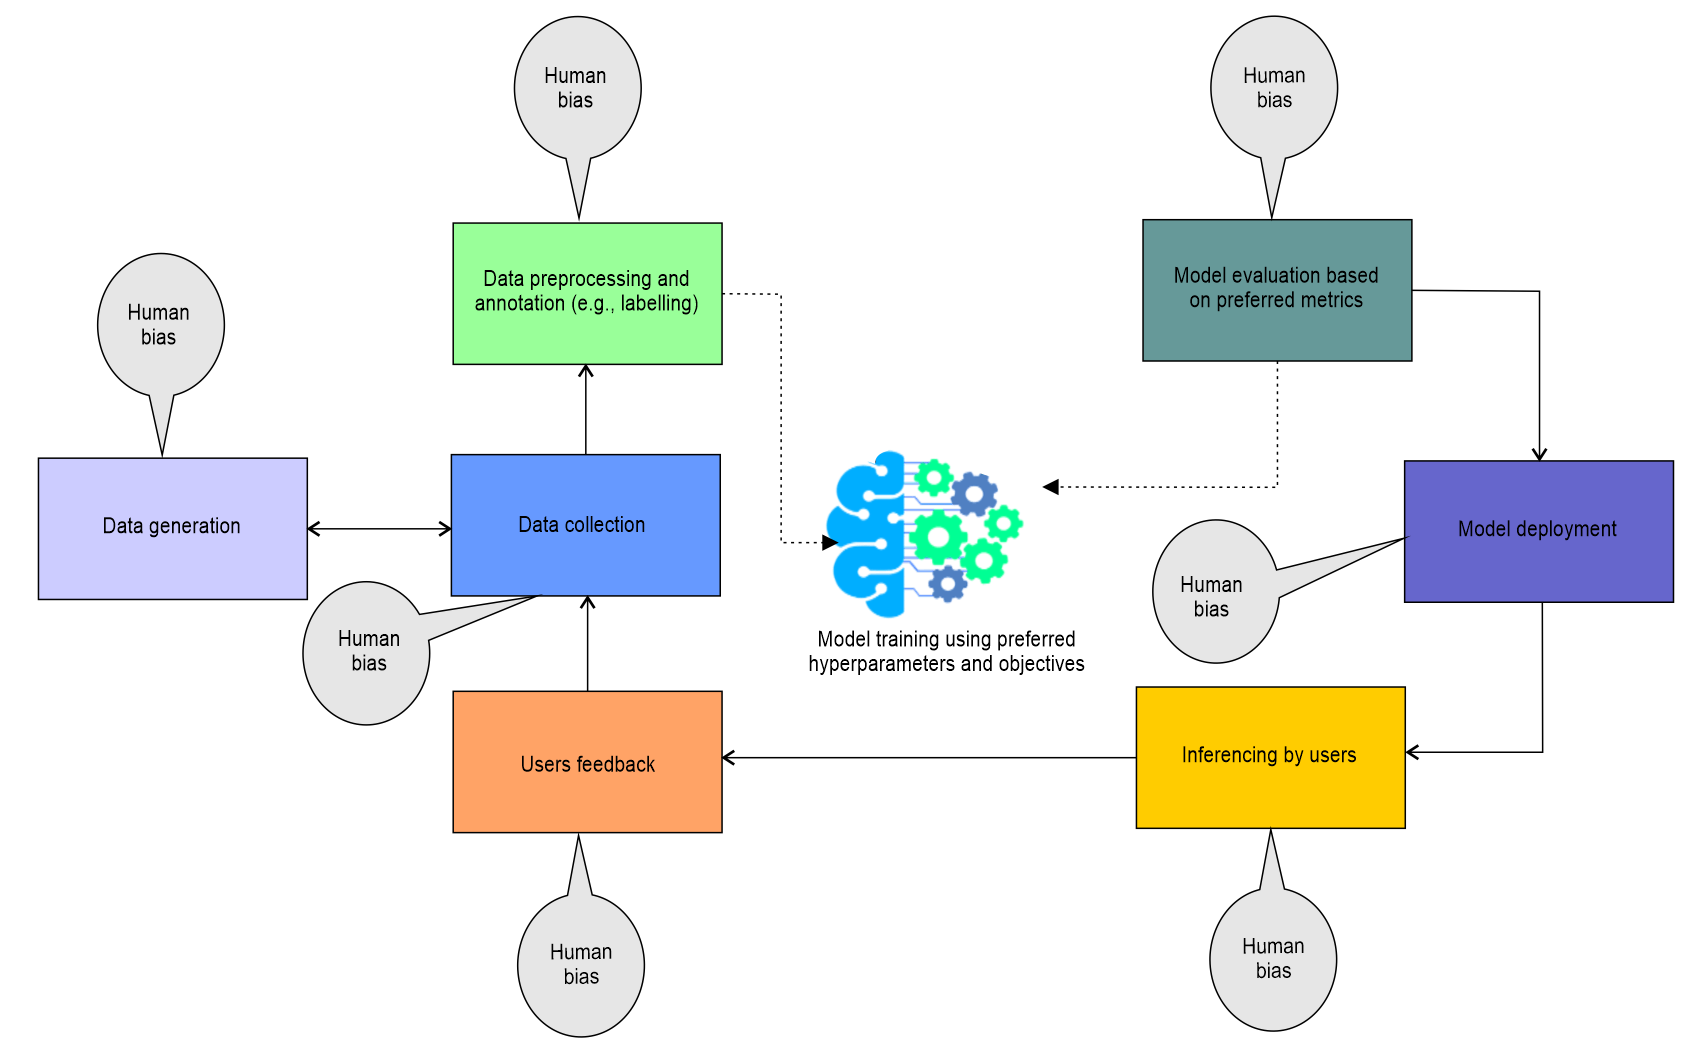
\includegraphics[scale=0.5]{images/bias_all.png}
        \label{fig:bias_in_stages}
	\caption{Bias involved in almost every stage in a typical ML pipeline} 
\end{figure}

\hspace*{3.5mm} Through several ante-hoc and post-hoc interpretability and explainability methods, we have seen uncovering algorithmic discrimination was relatively straightforward. However, since the generated explanations are based on statistical exercises, we cannot confidently say that decisions made by the CDSS are fair. Thus, when training a ML algorithm, it's important to aware of common human biases that can manifest in the data, so that proactive measures can be taken to mitigate their effects. %Through the thesis, employed several ante-hoc and post-hoc interpretability and explainability methods.
Through several ante-hoc and post-hoc interpretability and explainability methods, we already attempted opening several black-box ML models. We Identified correlated biomarkers. We have seen how a model makes certain predictions and generate domain knowledge via symbolic reasoning. However, it would not be fair to claim that the models trained would provide bias free~(for the simplicity, let's say fair) decision. Fighting against bias and discrimination has a long history in philosophy and psychology, and recently in ML~\cite{fairness_survey}. In order to achieve high degree of fairness by mitigating the discrimination, it is a prerequisite to know the definition and notions of fairness. 
%We observed that uncovering algorithmic discrimination was relatively straightforward. However, we generated the explanations based on mathematical and statistical exercises. 

%\section{Diagnosis Biases} %and Fairness of ML Systems}
%\label{chapter_9:preliminaries}
%In this section, we cover some preliminaries and concepts around definition and notions of fairness that will be used in subsequent sections. 

\iffalse
%\subsection{Fairness assessment}
\subsection{Fairness: algorithmic to philosophical fairness}
Although, philosophy and psychology have tried to define the concept of fairness long before it is first explored in the computer science realm, albeit there is no universal definition of fairness. In computer science most of the works focused on fairness constraints for algorithms. Some studies studied fairness definitions in political philosophy and tried to tie them to ML, especially they tied to fairness in algorithmic classification problems. We revisit some definitions and explanations from literature~\cite{fairness_survey} and~\cite{verma2018fairness}.

\vspace{-1mm}
\begin{definition}
    \textbf{Fairness in the context of decision-making}: fairness is the absence of any prejudice or favoritism toward an individual or groups based on inherent or acquired characteristics~\cite{fairness_survey}. 
\end{definition}
\vspace{-1mm}

\hspace*{3.5mm} Fairness definitions fall under different two different types: individual fairness vs. group fairness. The former, signifies giving similar predictions to similar individuals. In other words, similar individuals should be treated similarly. Literature~\cite{berk2017convex} has defined the individual fairness $f_i$ mathematically. For every cross pair $(x,y) \in S_{1},\left(x^{\prime}, y^{\prime}\right) \in S_{2}$, a model $F$ is penalized for how differently it treats $x$ and $x^{\prime}$ where $S_{1}$ and $S_{2}$ are different groups from the sampled population. It can be defined mathematically as follows~\cite{berk2017convex}: 

\vspace{-4mm}
\begin{align}
    f_{i}(F, S)=\frac{1}{n_{1} n_{2}} \sum_{\left(x_{i}, y_{i}\right) \in S_{1} \atop\left(x_{j}, y_{j}\right) \in S_{2}} d\left(y_{i}, y_{j}\right)\left(F \cdot x_{i}-F \cdot x_{j}\right)^{2},
\end{align}
\vspace{-4mm}

\hspace*{3.5mm} where $x^{\prime}$ is weighted by a function of $\left|y-y^{\prime}\right|$. On the other hand, group fairness states that ``on average, the two group's instances should have similar labels weighted by the nearness of the labels of the instances". Group fairness $f_g$ can be defined mathematically as follows~\cite{berk2017convex}: 

\vspace{-4mm}
\begin{align}
    f_{g}(F, S)=\left(\frac{1}{n_{1} n_{2}} \sum_{\left(x_{i}, y_{i}\right) \in S_{1} \atop\left(x_{j}, y_{j}\right) \in S_{2}} d\left(y_{i}, y_{j}\right)\left(F \cdot x_{i}-F \cdot x_{j}\right)\right)^{2}.
\end{align}
\vspace{-4mm}

\hspace*{3.5mm} In either way, these terms are based on anti-discrimination laws that define specific protected classes.
The third types of fairness, called subgroup fairness to obtain the best properties of the group and individual notions of fairness. It picks a group fairness constraint like equalizing false positive and asks whether this constraint holds over a large collection of subgroups. Besides, Verma et al.\cite{verma2018fairness} introduced other notions that promotes fairness through unawareness, awareness, and treatment equality scenarios:    

%\vspace{-2mm}
\begin{definition}
    \textbf{Fairness through awareness}: An algorithm is fair if it gives similar predictions to similar individuals. In other words, any two individuals who are similar with respect to a similarity metric defined for a particular task should receive a similar outcome~\cite{verma2018fairness}.
\end{definition}
\vspace{-4mm}
\begin{definition}
    \textbf{Fairness through unawareness}: an algorithm is fair as long as any protected attributes A are not explicitly used in the decision-making process~\cite{verma2018fairness}.
\end{definition}
\vspace{-4mm}
\begin{definition}
    \textbf{Fairness in treatment equality}: treatment equality is achieved when the ratio of false negatives and false positives is the same for both protected group categories~\cite{verma2018fairness}.
\end{definition}

%\vspace{2mm}
\begin{tcolorbox}[colback=white!3!white,colframe=gray!120!black,title=\faBook~Individual vs. group fairness]
    %INFO: \faBook \\
    \scriptsize{
    \textbf{Group fairness:} is defined by protected attributes receiving similar treatments or outcomes~(diagnosis in our case).\\
    \textbf{Individual fairness:} the goal of similar individuals receiving similar treatments or outcomes~(diagnosis in our case).
}
\end{tcolorbox}

%\vspace{2mm}
\begin{tcolorbox}[colback=white!3!white,colframe=gray!120!black,title=\faBook~Protected attributes]
    %INFO: \faBook \\
    \scriptsize{
    \textbf{Privileged protected attribute:} a value of a protected attribute indicating a group or class that has  been at systematic advantage during data collection or real-life scenario. \\
    \textbf{Protected attribute:} an attribute that divides the population into groups whose outcomes should have parity, e.g., patient race, gender, caste, and religion.
}
\end{tcolorbox}

\hspace*{3.5mm} Group fairness also emphasizes treating different groups equally, i.e., which group of individuals are at risk of experiencing harms or unfairness? Literature~\cite{verma2018fairness} defines relevant groups~(i.e., sub-populations) w.r.t sensitive features~(aka. sensitive patient attributes or protected attribute in a similar sense).
\fi 

%\subsection{Types of bias in ML systems}
\hspace*{3.5mm} Above discussed unfairness often evolve from numerous biases due to human involvement in the provision and curation of the data can make a model's predictions not only susceptible to bias but also erroneous outcome~\cite{futia2020integration}. Often false predictions from the bias can disproportionately impact in the diagnosis, which can tends a medical doctor to make wrong treatment. Eventually, biases are one of the main obstacles in fair decision making and can manifest in any part of the pipeline~\cite{GoogleBiasinMLPipeline,fairness_survey}: from data collections, feature selection, model training, setting hyperparameters, and the way results  interpreted to the end users, e.g., patients. Olteanu et al.~\cite{biasList} identified different types of biases. Bias in data can exist in many shapes and forms, some of which can lead to unfairness in different learning tasks~\cite{fairness_survey}. 

\begin{itemize}[noitemsep]
    \item \textbf{Reporting bias} - occurs when the frequency of events, properties, and outcomes captured in a dataset does not accurately reflect their real-world frequency~\cite{GoogleBiasList}, e.g., in sentiment-analysis, majority of reviews in the training dataset reflect extreme opinions - a reviewers who either loved or hated a book, making the data imbalanced, i.e., biased towards negative or positive sentiments. Consequently, the model would be less effective to correctly predict sentiment of reviews. 
    \item \textbf{Automation bias} - a tendency to favor results generated by a ML model over other research, irrespective of the error rates of each~\cite{GoogleBiasList}, e.g., to train until model's precision and recall are both 15\% higher than a previous approach.
    \item \textbf{Selection bias} - when the samples selection does not reflective of their real-world distributions~\cite{GoogleBiasList}. 
    \item \textbf{Coverage bias} - occurs if the data is not selected in a representative fashion\cite{GoogleBiasList}, e.g., a model is trained to predict the loan  outcomes based on the previously successful loan applications. This, however, implicitly means that customers whose applications were rejected were not considered, i.e., the defaulter group was not represented in the training data.
    \item \textbf{Sampling bias} - occurs mainly when the distribution of the training data does not reflect the actual environment the ML model will be running in. For example, for a self-driving car scenario, if the training data (e.g., video) is prepared based on daylight video, the data is still biased since there is no night time samples. Other discriminatory bias can be introduced into data too, e.g., unbalanced data can create biases against underrepresented groups. 
    \item \textbf{Experimenter's bias} - often data scientists build a model on unconsciously process data in ways that affirm preexisting beliefs and hypotheses~\cite{GoogleBiasList}. Nonetheless, selection of algorithms or hyperparameters are also introduce experiments bias. 
\end{itemize}

\hspace*{3.5mm} Although statistically bias means an inaccurate representation of what is true w.r.t the underlying population, from the social context, it is a preference for an outcome or group of people, whether it is fair or unfair. Since fairness is a broad term, we assume bias means unfair or unwanted diagnosis decision made by the CDSS. Hence, we'll emphasize on understanding different types of bias, identifying them, and evaluating the measurement of biases, before we mitigate them. Although decisions made by the model has to be fair, it is not possible to say how interpretable and fair our approach is, unless the interpretability and fairness\footnote{\textbf{RQ5}: How to score a `black-box' model on fairness and transparency, e.g., why did the model behave in a certain way?} are assessed. Given that the model can explain how it works, how do we know whether: i) the explanations are reliable?, ii) users can have a realistic understanding and human-level interpretability?, iii) what would we do if the patient thinks the model is not trustworthy? We answer above questions by combining the predictions and knowledge from the model with the decision reasoning to generate interpretable and fair decision rules. 

%\hspace*{3.5mm} The rest of the chapter is structured as follows: 
%\cref{chapter_9:preliminaries} covers preliminaries and concepts that will be used in other sections in this chapter. \cref{chapter_9:mm} describes the overall approach for mitigating different types of unfairness before assessing the fairness. \Cref{sec:rule_gen_inter} covers generating and interpreting fair decision rules. \Cref{chapter_9:conclusion} provides explanations of the importance and relevance of the study reported, highlights the limitations and discuss  future works before concluding the chapter. 

\section{Methods} \label{chapter_9:mm}
Although fairness is an incredibly desirable quality from both clinical, technological, or philosophical side, it would be surprisingly difficult to make the CDSS fully fair. We argue saying that fairness is the process of understanding bias introduced by the data, and ensuring the model provides equitable predictions across all individual and demographic groups. When it comes to fairness literature and tools, they suggest that the fairness can be measured at different points in a ML pipeline: either on the training data or on the learned model, so that unfairness mitigation attempts can be taken. 

\iffalse
\subsection{Fairness assessment of CDSS}
There are many approaches to conceptualizing fairness. In Fairlearn, we follow the approach known as group fairness, which asks: Which groups of individuals are at risk for experiencing harms?

The relevant groups (also called subpopulations) are defined using sensitive features (or sensitive attributes), which are passed to a Fairlearn estimator as a vector or a matrix called sensitive\_features (even if it is only one feature). The term suggests that the system designer should be sensitive to these features when assessing group fairness. Although these features may sometimes have privacy implications (e.g., gender or age) in other cases they may not (e.g., whether or not someone is a native speaker of a particular language). Moreover, the word sensitive does not imply that these features should not be used to make predictions – indeed, in some cases it may be better to include them.

Fairness literature also uses the term protected attribute in a similar sense as sensitive feature. The term is based on anti-discrimination laws that define specific protected classes. Since we seek to apply group fairness in a wider range of settings, we avoid this term
\fi 

%\subsection{Unfairness mitigation}
\hspace*{3.5mm} Bias mitigation algorithms attempt to improve the fairness metrics by modifying the training data, the learning algorithm, or the predictions. So, unfairness can be mitigated during the pre-processing, in-processing, and post-processing, respectively. In both assessment and mitigation scenarios, fairness is quantified using disparity metrics. However, this study does not yet considered the external validation in a clinical setting. Rather in our approach, we try to improve the decision fairness by mitigating the biases in 3 different ways: i) mitigating sampling biases before the model training, ii) reducing prediction biases, and iii) model selection biases, before generating fair decision rules for the cancer diagnosis. 
%We try to mitigate the biases in both binary and multiclass classification settings. 

\begin{sidewaysfigure*}
	\centering
	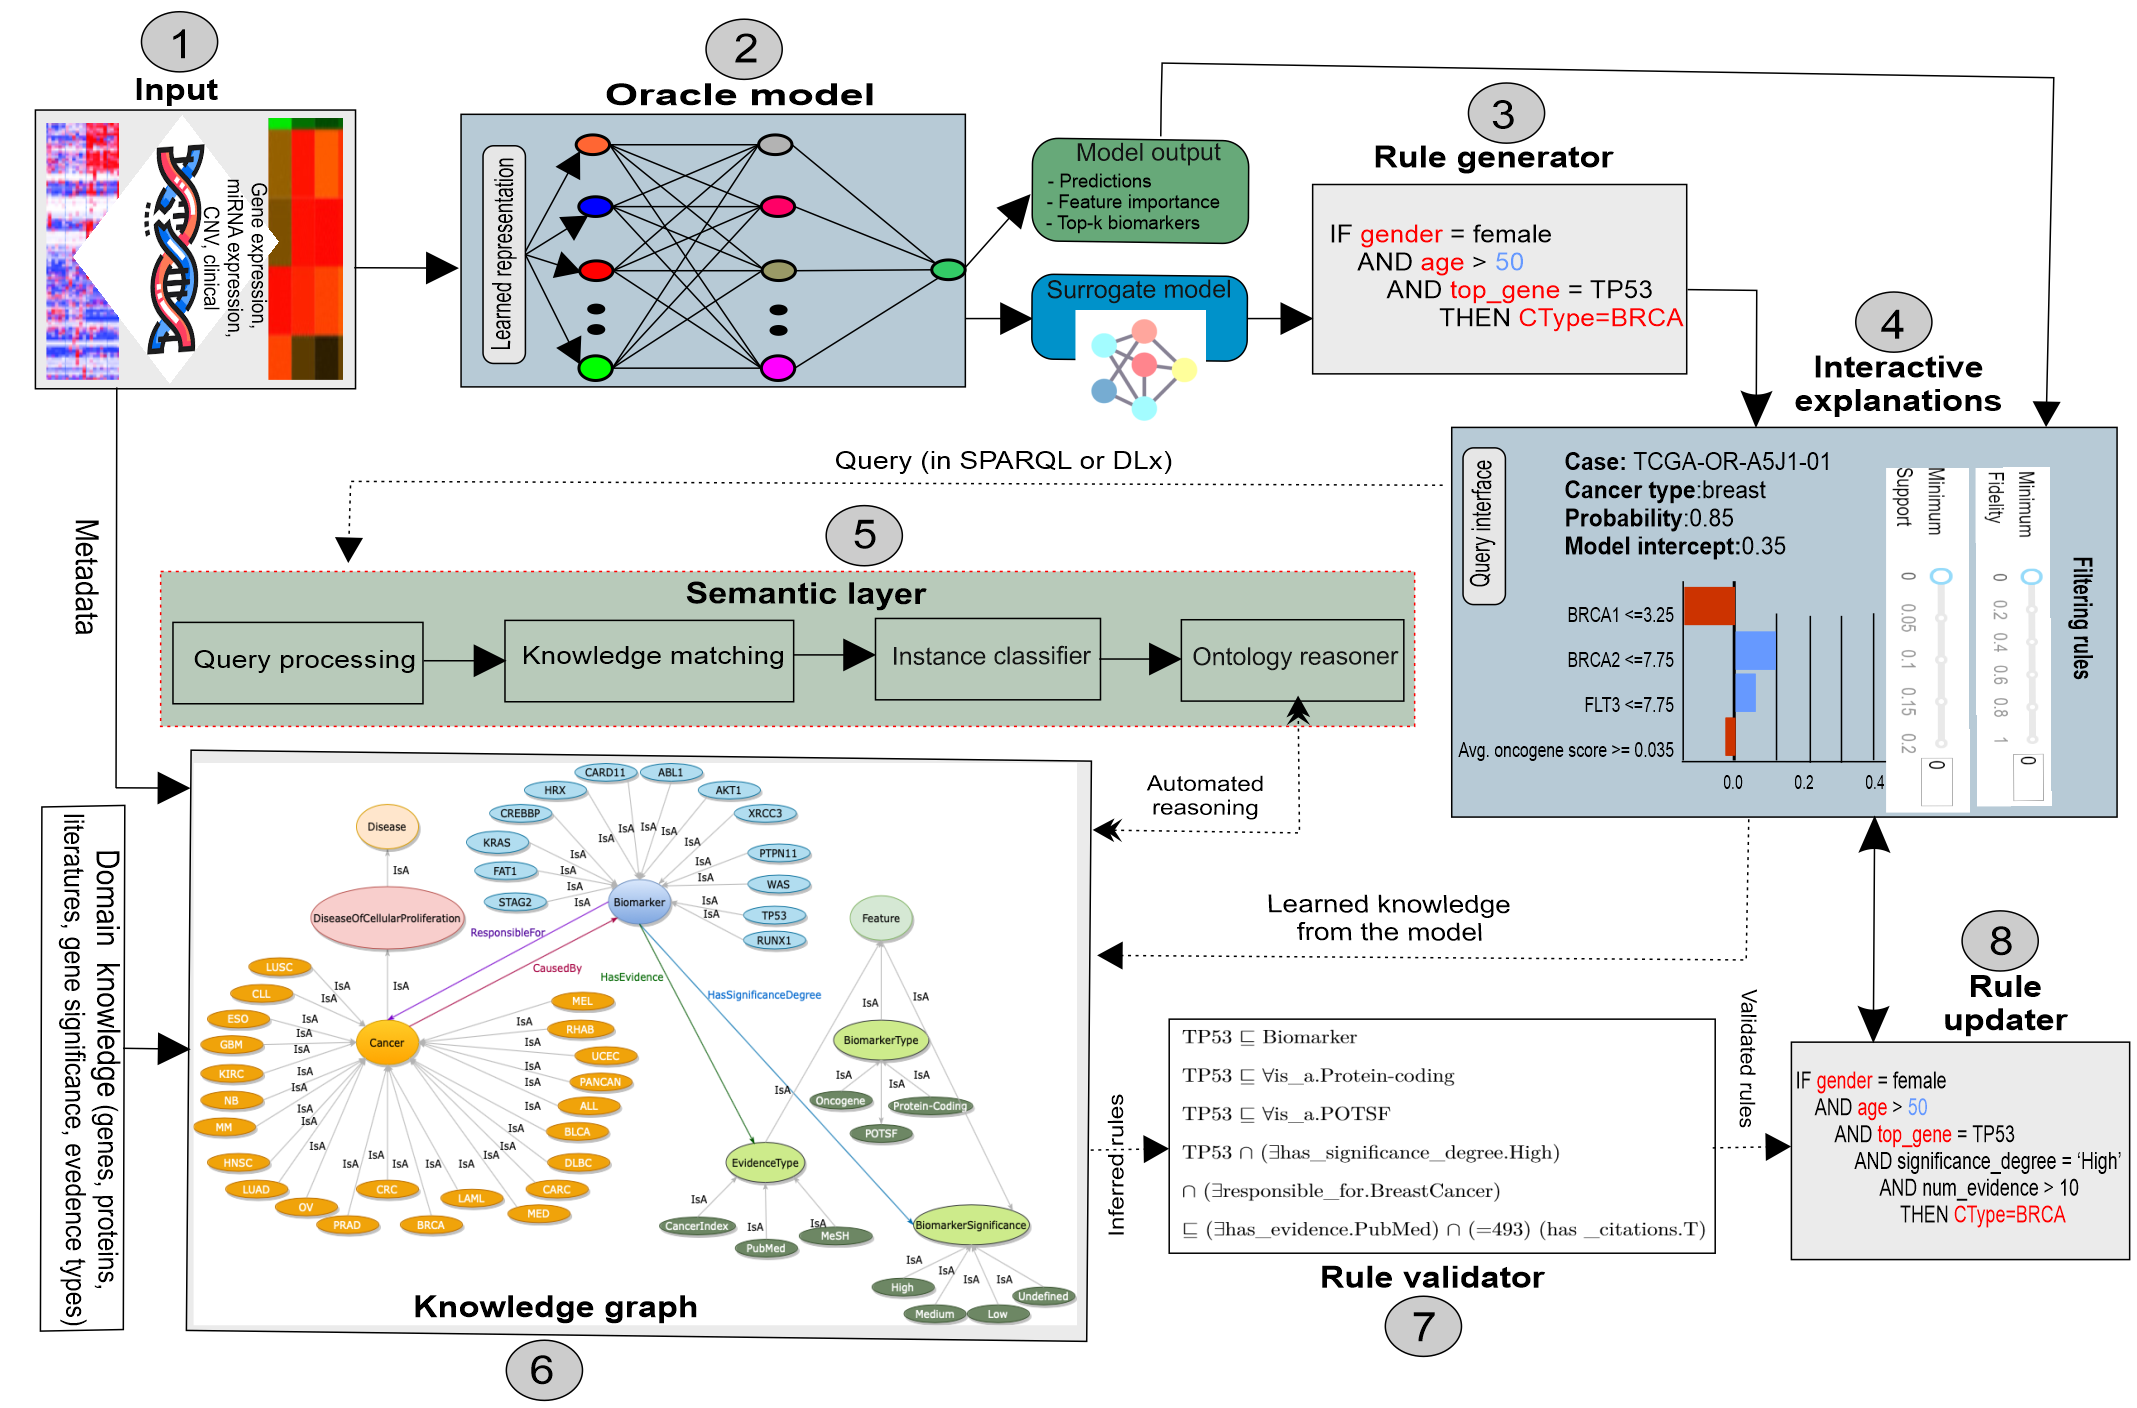
\includegraphics[width=\linewidth]{images/reasoning_wf.png}
    \label{fig:nsreasoning}
	\caption[Overview of fair decision rules generation based symbolic reasoning]{Overview of fair decision rules generation based symbolic reasoning. The reasoner reasons about the predictions and decision rules made by the model based on ontological concepts and provides additional information back to the interactive visualization module.} 
	\vspace{-4mm}
\end{sidewaysfigure*}

\subsection{Mitigating sampling biases}
%\subsubsection{Mitigating heterogeneity}
Sampling bias arises in the data collection or preparation steps when non-random sampling of subgroups occurs. As a consequence, trends estimated for one population may not generalize to data collected from a new population~\cite{mehrabi2019survey}. Kim DW. et al.~\cite{kim2019design}, has suggested to follow 4 fundamental methodological features for real clinical validation of AI performance in real-world practice, where for training ML algorithms with the data based not only on internal validation but also external validation, data are diagnostic cohort design instead of diagnostic case-control design, iii) data are coming from multiple institutions, iv) in a prospective manner. These are among fundamental methodological features recommended for clinical validation of AI performance in real-world practice~\cite{kim2019design}. Therefore, when training a ML algorithm, it's important to aware of common human biases that can manifest in the data, so that proactive steps can be taken to mitigate their effects. Data from different institutions creates several challenges, e.g., heterogeneity, although data used from one source can lead to non generalizable models. However, heterogeneity impedes in better learning/training, while the out-of-distribution may often tend the model to make wrong predictions, which is not acceptable in real clinical setting. 

\hspace*{3.5mm} Since biases involve almost every single steps in a ML pipeline, we can't eliminate biases completely even it is from a single source. However, at least, we have to make sure that data is being produced at each institute under/with the same modality or technology. As outlined in \cref{tab:platforms}, miRNA expression, mutations, DNA methylation, GE, and copy numbers~(at gene and probe-level) data used in this study are based on GRCh37~(hg19) and GRCh38~(hg38) version\footnote{GRC = Genome Reference Consortium}~\cite{gao2019before} reference genomes and generated with different platforms. GRCh38 is an improvement over GRCh37 from the genome assembly aspect, which yields more reliable genomic analysis results~\cite{guo2017improvements}. GRC38 offers overall more accurate analysis of human sequencing data by producing fewer false positive structural variants. Both versions were ‘harmonized’ by the genomic data commons~(GDC) as they are mostly consistent\cite{guo2017improvements}. To mitigate probable biases, we excluded the samples from hg19 version.  

\begin{table}
    \centering
    \scriptsize
    \caption{Platforms and reference genomes used in TCGA}
    \label{tab:platforms}
    \vspace{-2mm}
    \begin{tabular}{l|l|l} 
        \hline
        \textbf{Input data} & \textbf{Platform} & \textbf{Reference genome}  \\ 
        \hline
        \multirow{2}{*}{DNA methylation}  & Infinium Human Methylation 27K & GRCh38  \\ 
        \cline{2-3}
                                               & Infinium Human Methylation 450K & GRCh37 \\ 
        \hline
        \multirow{2}{*}{Gene expression}       & Agilent 244K Custom Gene Expression & GRCh38 \\ 
        \cline{2-3}
                                               & Affymetrix Human Genome U133A 2.0 Array & GRCh37 \\ 
        \hline
        \multirow{2}{*}{miRNA expression}      & Agilent Human miRNA Microarray & GRCh38 \\ 
        \cline{2-3}
                                               & Illumina Genome Analyzer miRNA Sequencing & GRCh37  \\ 
        \hline
        \multirow{2}{*}{Copy numver variation} & \multirow{2}{*}{Illumina HiSeq}           & GRCh38  \\
                                               &                                           & GRCh37 \\ 
        \hline
    \end{tabular}
    \vspace{-2mm}
\end{table}

\hspace*{3.5mm} The DNA methylation data in this study was derived from one of two array-based platforms: Infinium Human Methylation 27K~(HM27) and Infinium Human Methylation 450k~(HM450). As literature~\cite{pidsley2013data} has argued, 450K includes 90\% of the 27k probes and has far greater coverage. Further, it has been discovered the range of data for each dataset to be slightly different. Hence, it is not recommended to combine these together and using the shared probes. As such, literature~\cite{pidsley2013data} recommend applying normalization in case we still want them combined. Subsequently, we retrain the model based on the samples from 450K platform only, in order to mitigate the probable biases. 
Apart from the heterogeneity, sampling bias also taken into consideration. Since, gender is an important feature or variable for certain cancer types like breast and ovarian cancer, this variable is naturally and statistically not significant for the male patients. In the symbolic-reasoning step, this feature can be identified as a discriminating bias towards a certain group or sub-group of patients, given that patient identify is known to the doctor. However, due to nature of the data and lack of clinical validation, we could not perform such bias mitigation. 

\hspace*{3.5mm} After mitigating above biases, lightweight pre-processing was performed by reweighing and the adversarial debiasing algorithms. A potential advantage of employing reweighing is that it only changes weights applied to training samples, leaving the feature or label values intact. Therefore, fairness literature recommends it as a preferred option given that the CDSS does not expect for value changes, i.e., adversarial samples. On the other hand, adversarial debiasing algorithm learns a classifier to maximizes the prediction accuracy as well as reduces an adversary's ability to determine the protected attribute from the predictions. Since our CDSS is sensitive to protected attribute too, this approach is expected to lead to a fair classifier as the predictions cannot carry any group discrimination information that the adversary can exploit. 

\subsection{Reducing prediction biases}
Fairness in both data and ML algorithms is critical to building safe and responsible AI-guided systems, in almost all the domain, especially healthcare. While accuracy, precision, recall, F1, or MCC are a few metrics for evaluating the accuracy of a ML model, fairness gives us a way to understand the practical implications of a deployed model in real clinical setting. Human involvement in the provision and curation of data can make a model's predictions not only susceptible to bias but also erroneous outcome. 
%\subsection{Fairness of the decision and diagnosis}
%\subsection{Explanations with SHAP}

\begin{figure}[h]
\centering
	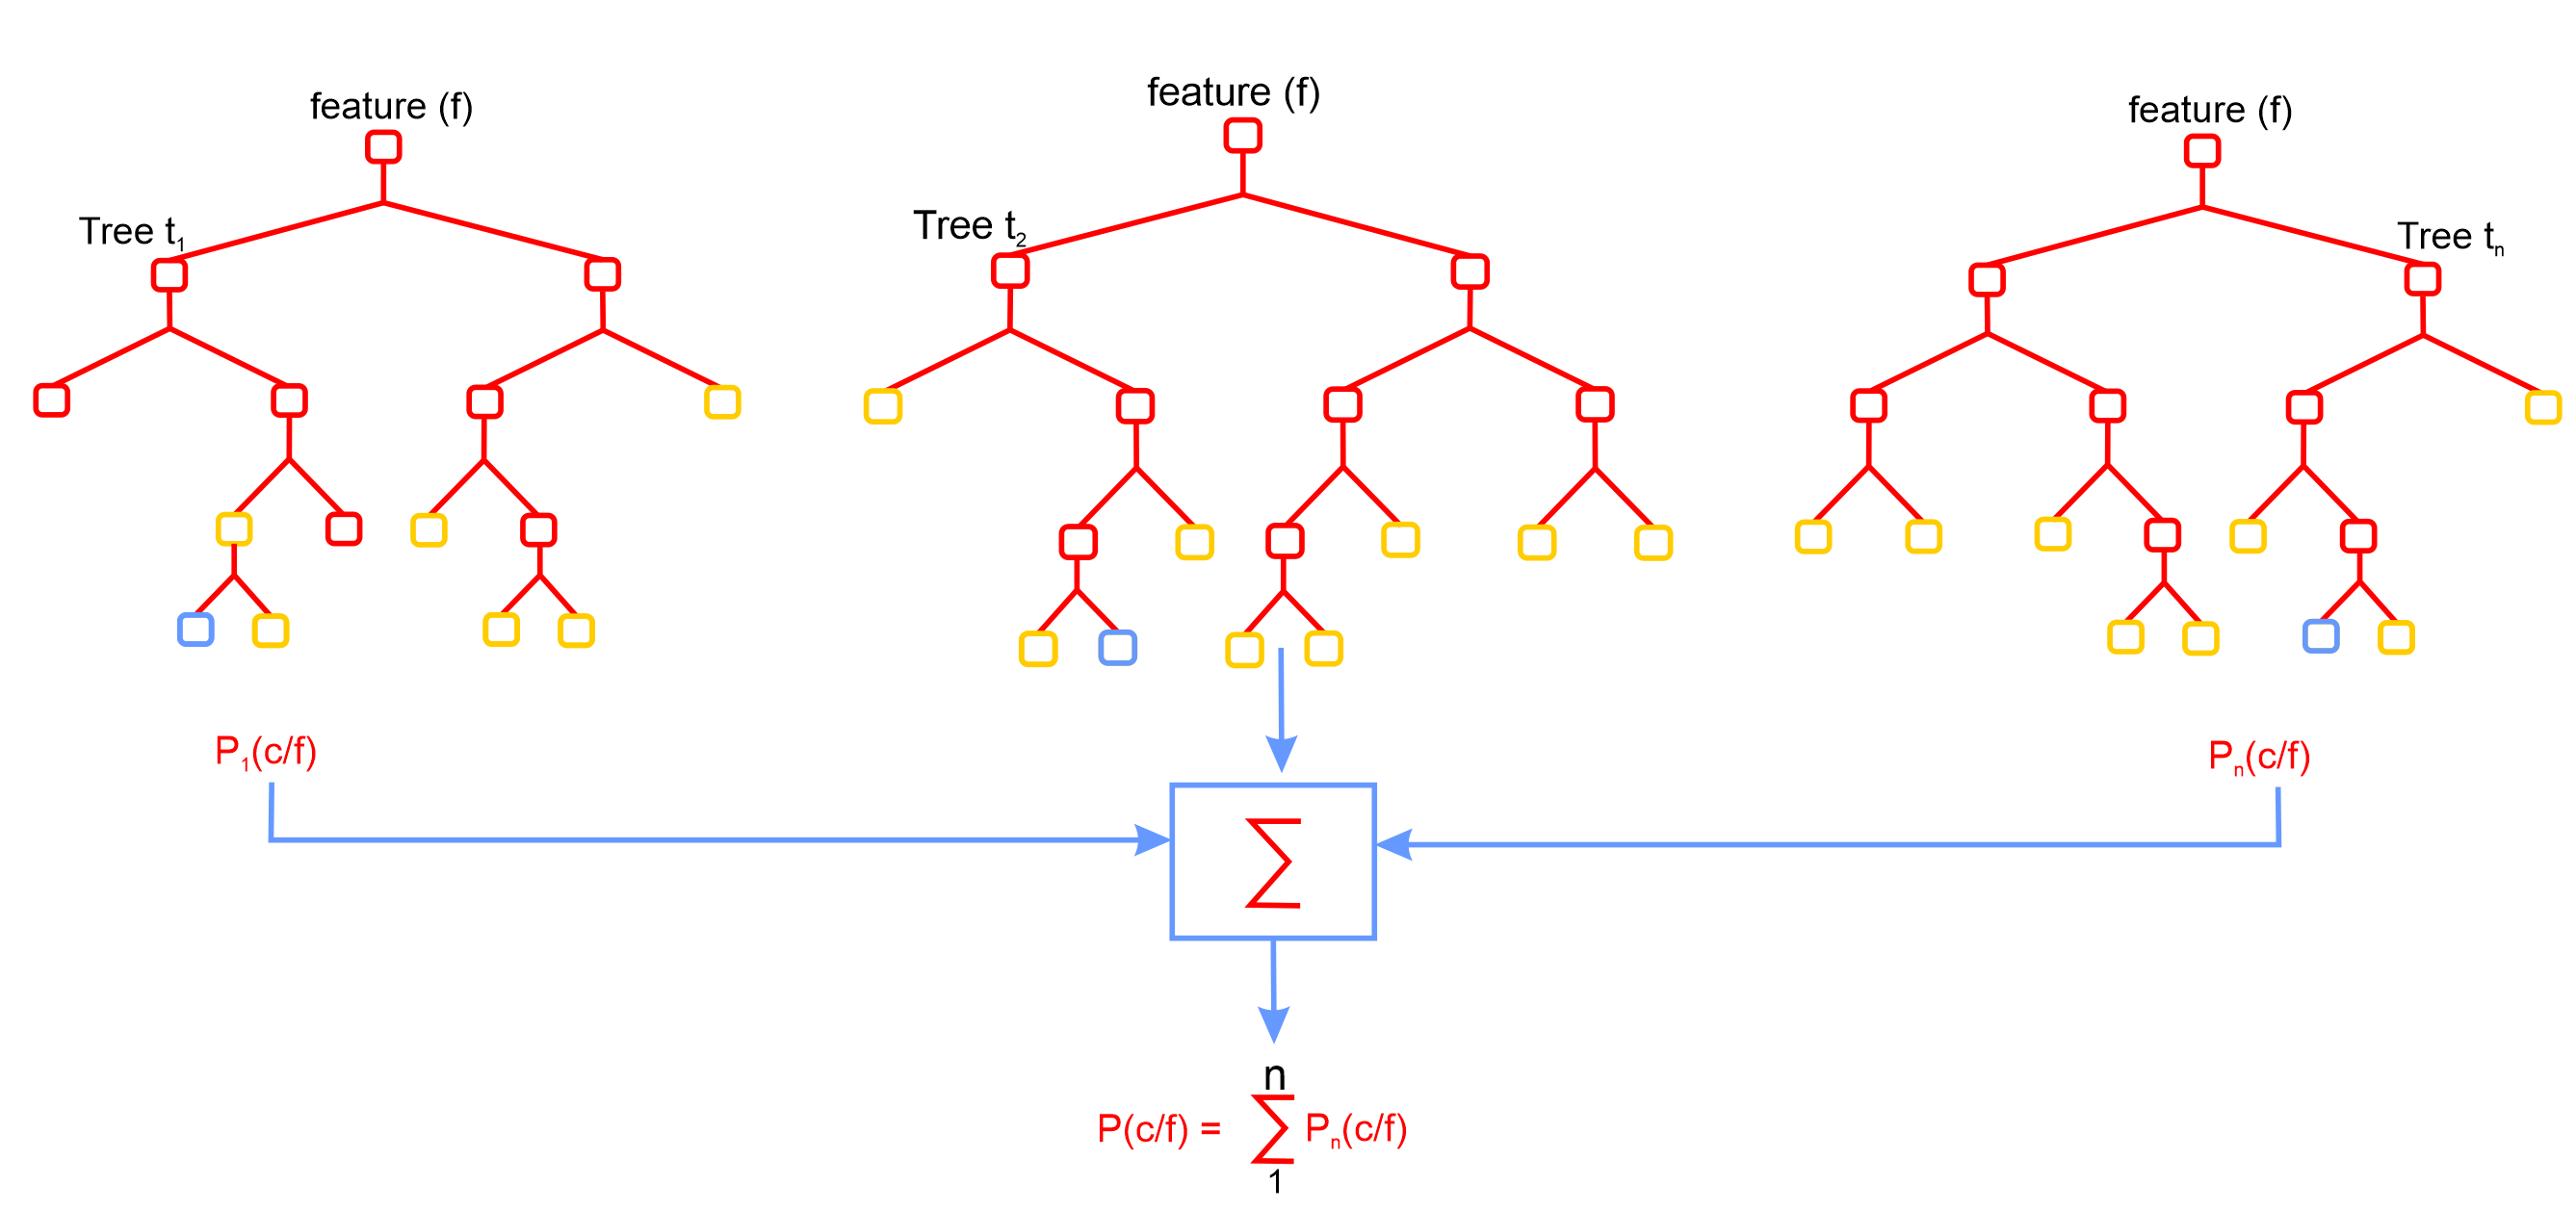
\includegraphics[width=0.8\textwidth]{images/rf_tree.png}
	\caption[Random forest and its assembling technique explained]{Random forest and its assembling technique explained~\cite{karim2018scala}} 
	\label{fig:RF_model}
\end{figure}

\hspace*{3.5mm}We employ SHAP to provide the explanations of the predictions made by the random forest~(RF) model. RF is an ensemble technique that takes a subset of observations and a subset of variables to build decision trees that creates ensemble of decision trees. A RF model first builds decision trees then integrates them to get a more accurate and stable prediction. This is a direct consequence, since by maximum voting from a panel of independent juries, we get the final prediction better, fair, and trustworthy than the best jury. \Cref{fig:RF_model} shows a RF and its assembling technique. There is no definite answer to if feature importance~(FI) should be computed while providing the explanations on the training set or test set. However, Molnar et al.~\cite{molnar2019interpretable} has the following recommendation: 

\begin{itemize} [noitemsep]
    \item If we want to measure how much the model itself depends on each feature making predictions? The FI should be computed on the training set.
    \item If we are require to measure how much each feature contributes to the performance of the model on unseen data, the same should be computed on the test set. 
\end{itemize}

\hspace*{3.5mm} However, in our case, we consider both approaches: while the former is employed to assess the model during the training time, whereas the latter is applied to generate the explanation. First, we compute the permutation importance in which top features are given more importance and those towards the bottom matter least.
The first number in each row shows how much model performance decreased with a random shuffling, based on the `accuracy' as the performance metric. 
However, due to randomness, model's performance changes from a shuffling a column. Therefore, we measure the amount of randomness in our permutation importance calculation by repeating the process with multiple shuffles. The number after the $±$ measures how performance varied from one-reshuffling to the next. In our case, the most important feature/biomarker found based on permutation importance was `HMGN2P46'. %That seems sensible. Soccer fans may have some intuition about whether the orderings of other variables are surprising or not.

\begin{figure}[h]
\centering
	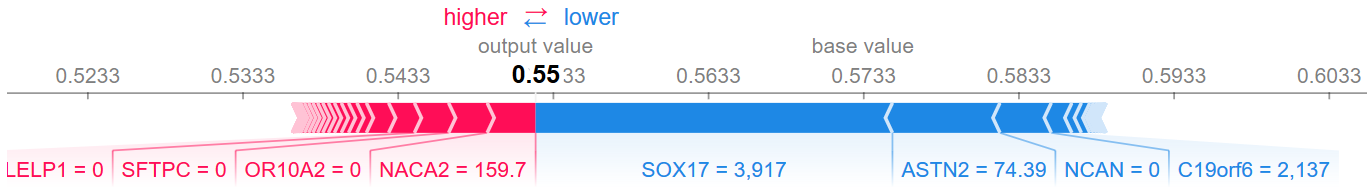
\includegraphics[scale=0.8]{images/shap.png}
	\caption{Clinical feature contribution for a prediction: red pushes predictions higher, blue ones lower} 
	\label{fig:shap}
	\vspace{-2mm}
\end{figure}

\hspace*{3.5mm} On the other hand, SHAP gives very different feature importance, as show in in \cref{fig:shap}, where a base value that indicates the direction of the first prediction made by the RF model and shows how much each feature is pushing the model's output from the base value\footnote{The average model output over the training dataset passed} 0.55 to the predicted output. Features pushing the prediction higher are shown in red; those pushing the prediction lower are in blue.

\begin{figure*}[h]
\centering
	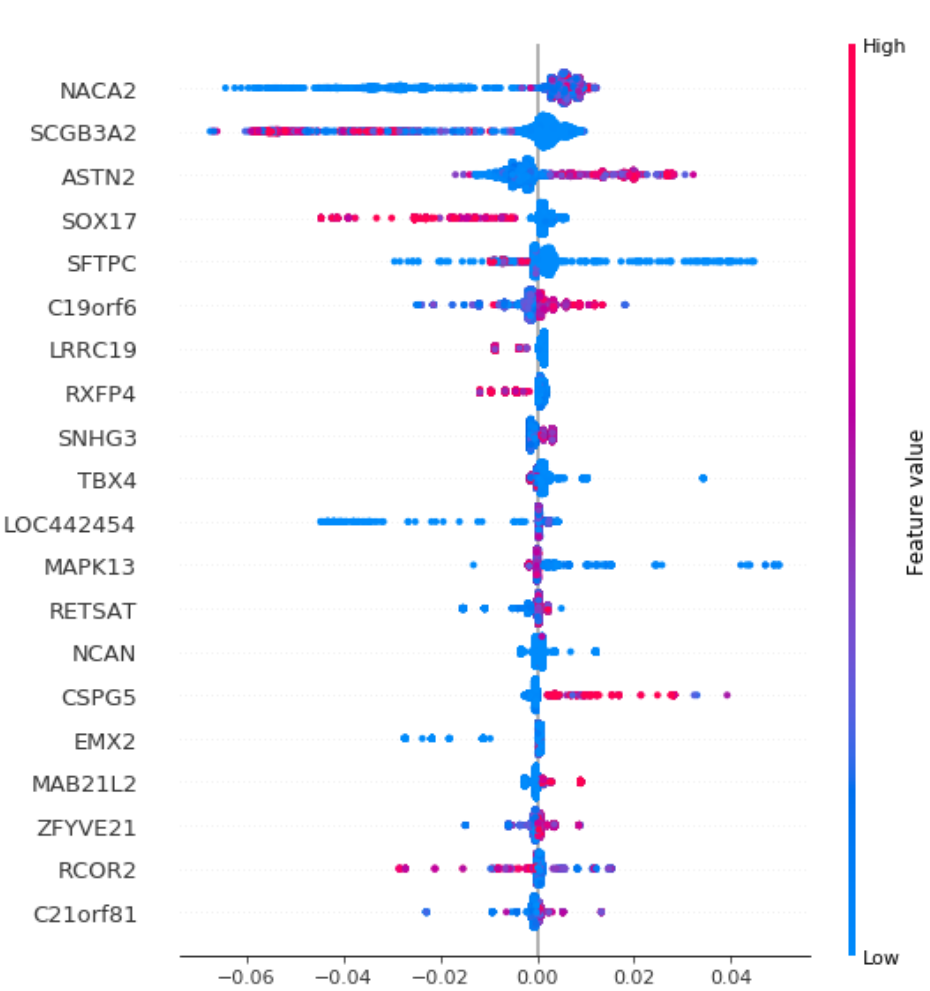
\includegraphics[scale=0.8]{images/fi.png}
	\caption[Clinical features ordered by ascending importance]{Clinical features ordered by ascending importance on the y-axis~(dots represent SHAP values)} 
	\label{fig:shap_FI}
	\vspace{-2mm}
\end{figure*}

\hspace*{3.5mm} Further, to get an overview of which biomarkers are most important for the RF model, we plot the SHAP values of each feature for each sample. The plot in \cref{fig:shap_FI} sorts features by the sum of SHAP value magnitudes over all the samples, shows the distribution of the impact of each feature on the model output, and gives the top-20 common biomarkers, where red represents high feature values, blue low. This reveals, e.g., that a low NACA2~(low GE value) lowers the predicted value across 33 cancer types. Since the common biomarkers predicted by VGG16 and RF are very different, a more detailed analysis of biological signaling pathways is further required to validate these findings. 

%\subsection{Increasing the fairness by reducing biases}
\subsection{Mitigating model selection bias}
In the previous chapters, we have created several snapshot models before generating the best model. However, worse snapshot can contaminate the overall predictive powers of the ensemble model itself. Therefore, it is important to take into consideration the model selection bias given. % the fact that we tried to evaluate the best performing model and subsequently the CDSS was backed by it.
Nevertheless, full convergence to best hyperparameters is often not necessary, as a best-fitted model will perform better on unseen data. To mitigate model selection bias,  WeightWatcher~\cite{martin2019traditional} library is used in following two levels: 

\begin{itemize}[noitemsep]
    \item \textbf{Level 1 } - top-5 snapshots models were selected to generate the full model
    \item \textbf{Level 2} - only the best model is selected for the final ensemble. 
\end{itemize}

\hspace*{3.5mm} In level 2, WeightWatcher is used to compare top models before choosing the one with the lowest log norm and highest weighted alpha. A low weighted/average log-norm signifies better generalization of network weights, where a pretrained model having low average log-norm will most likely show generalization capability and perform better on unseen data~\cite{martin2019traditional}. 

\begin{figure*}[h]
	\centering
	\begin{subfigure}{.48\linewidth}
		\centering
		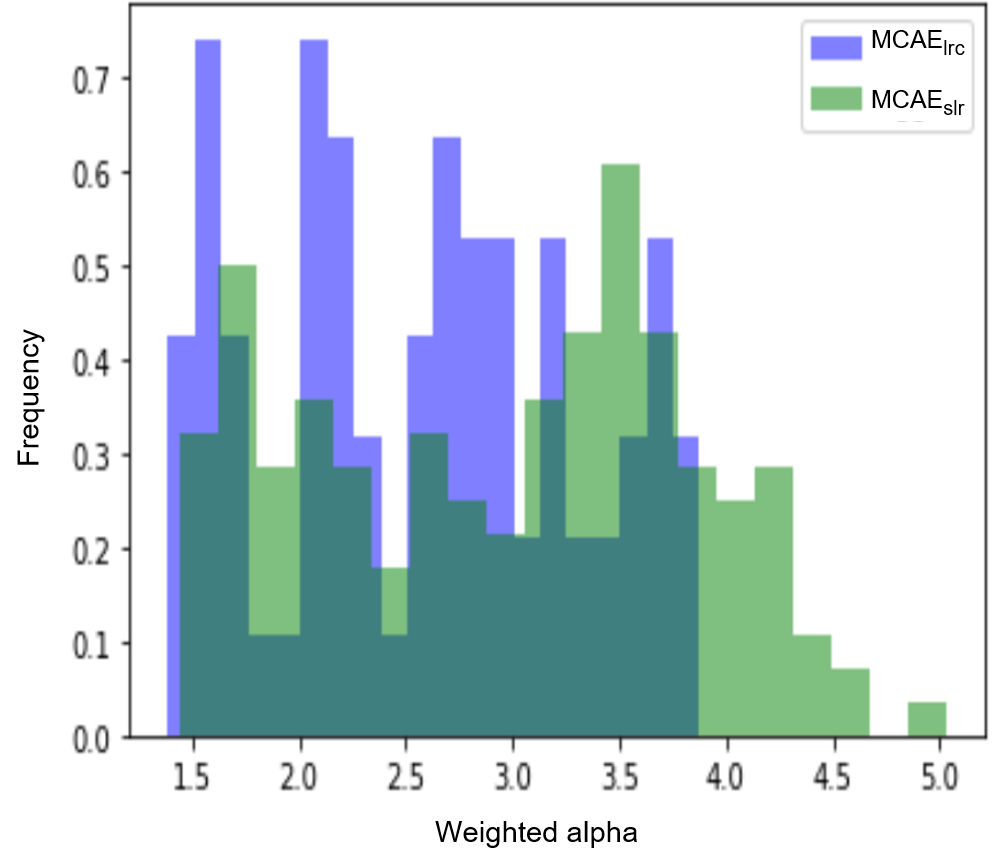
\includegraphics[width=0.8\linewidth,height=45mm]{images/w1.png}
		\caption{$F_{1}$ vs. $F_{2}$ in terms of weighted alpha}
        \label{fig:ww1}
	\end{subfigure}
	\begin{subfigure}{0.48\linewidth}
		\centering
		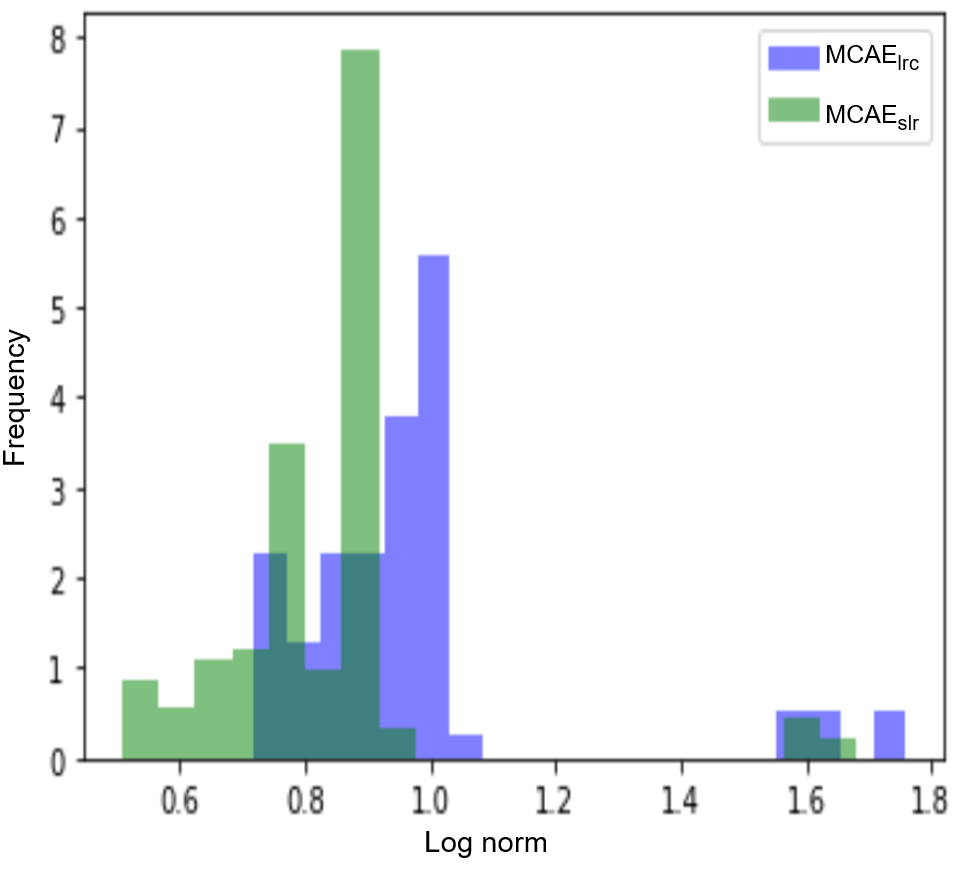
\includegraphics[width=0.8\linewidth,height=45mm]{images/w2.png}
		\caption{$F_{1}$ vs. $F_{2}$ in terms of log norm}
        \label{fig:ww2}
	\end{subfigure}
	\caption[Using WeightWatcher to compare and choose the best models]{Using WeightWatcher to compare $MCAE_{lrc}$ vs. $MCAE_{slr}$ and choose the best model}
	\label{fig:weight_watch}
	\vspace{-2mm}
\end{figure*}

\hspace*{3.5mm} \Cref{fig:weight_watch} shows choosing the better model between $MCAE_{lrc}$ vs. $MCAE_{slr}$ with WeightWatcher in terms of weighted alpha and log norm. The weighted alpha is based on the `power law' (or the `scaling law') principle, which states that a relative change in one quantity results in a relatively proportional change in another~\cite{clauset2009power}. A `power law' distribution has the form $Y = kX^{\alpha}$, where, $X$ and $Y$ are variables of interest, $\alpha$ is the law's exponent, and $k$ is a constant~\cite{clauset2009power}. Any inverse relationship like $Y=X^{-1}$ is also a power law because a change in one quantity results in an adverse change in another.

\iffalse
\subsection{Assessing fairness of diagnosis}
 Since our CDSS is concerned with both individual and group fairness, we compute both SampleDistortionMetric and  BinaryLabelDatasetMetric metrics. Besides, we computed the generalized entropy index for both individual and group fairness setting. However, for the simplicity, we perform the bias mitigation in a binary classification setting, i.e., first screening, where the model predicts if a group of patients have cancer or not, before predicting the types of cancer. As outlined earlier, we show two examples of such bias mitigation, based on reweighing and adversarial debiasing algorithms. 

\hspace*{3.5mm} In \cref{fig:debiases_1}, `female' is the privileged group, while male is the unprivileged group. As outlined the diagnosis accuracy after the bias mitigation changed from 91\% to 93\%. While in case of `white' privileged group~(and `black' unprivileged group), the diagnosis accuracy after the bias mitigation reduced from 93\% to 89\%. Although, bias against unprivileged group was reduced, it is still a acceptable level, reducing a chance of wrong diagnosis.  

\begin{figure*}[h]
	\centering
	\begin{subfigure}{.48\linewidth}
		\centering
		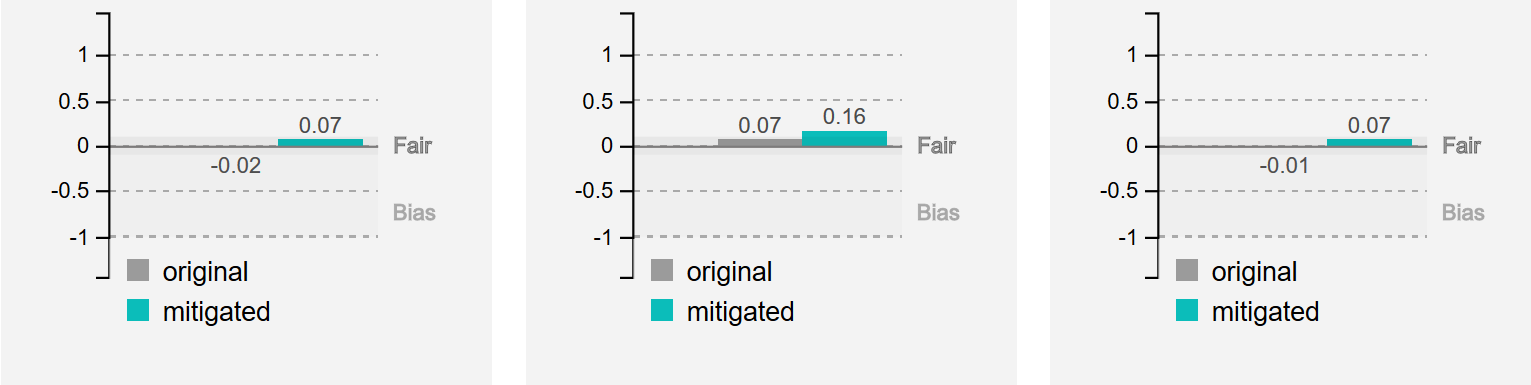
\includegraphics[width=\linewidth,height=25mm]{images/debias_1.png}
		\caption{Privileged male and unprivileged female groups}
		 \label{fig:debias_1}
	\end{subfigure}
	\begin{subfigure}{0.48\linewidth}
		\centering
		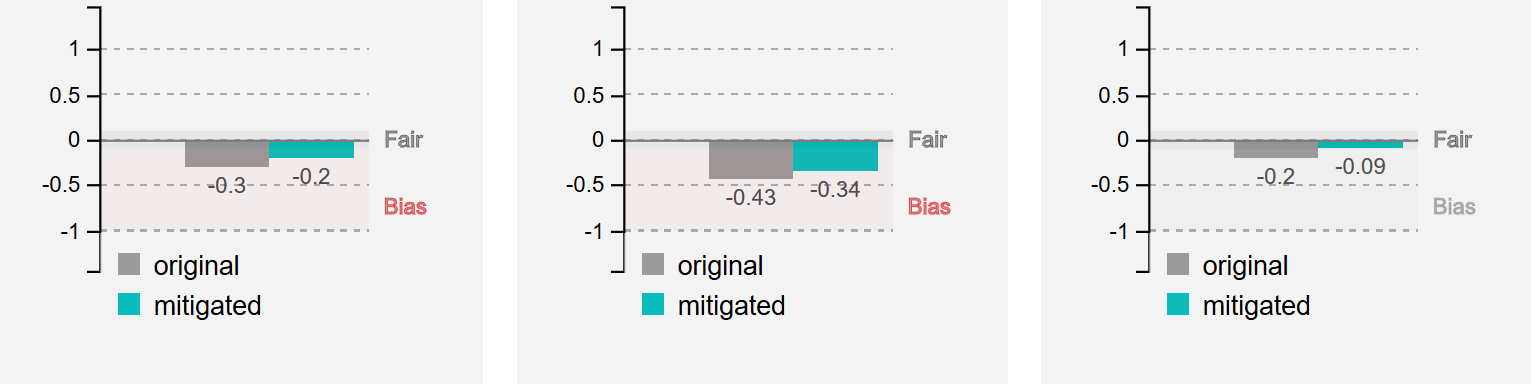
\includegraphics[width=\linewidth,height=25mm]{images/debias_2.png}
		\caption{Privileged 'white' and unprivileged 'black' groups}
        \label{fig:debias_2}
	\end{subfigure}
	\caption[Bias mitigation using reweighing algorithm]{Bias mitigation using reweighing algorithm, where statistical parity difference, equal opportunity difference, and average odds difference are shown}
	\label{fig:debiases_1}
	\vspace{-2mm}
\end{figure*}

\hspace*{3.5mm} In \cref{fig:debiases_2}, `black' is the privileged group, while `white' is the unprivileged group. As outlined the diagnosis accuracy after the bias mitigation changed from 92\% to 94.5\%. While in case of `white' privileged group~(and `black' unprivileged group), the diagnosis accuracy after the bias mitigation reduced from 94\% to 91\%. Although, bias against unprivileged group was reduced, it is still a acceptable level, reducing a chance of wrong diagnosis.  

\begin{figure*}[h]
	\centering
	\begin{subfigure}{.48\linewidth}
		\centering
		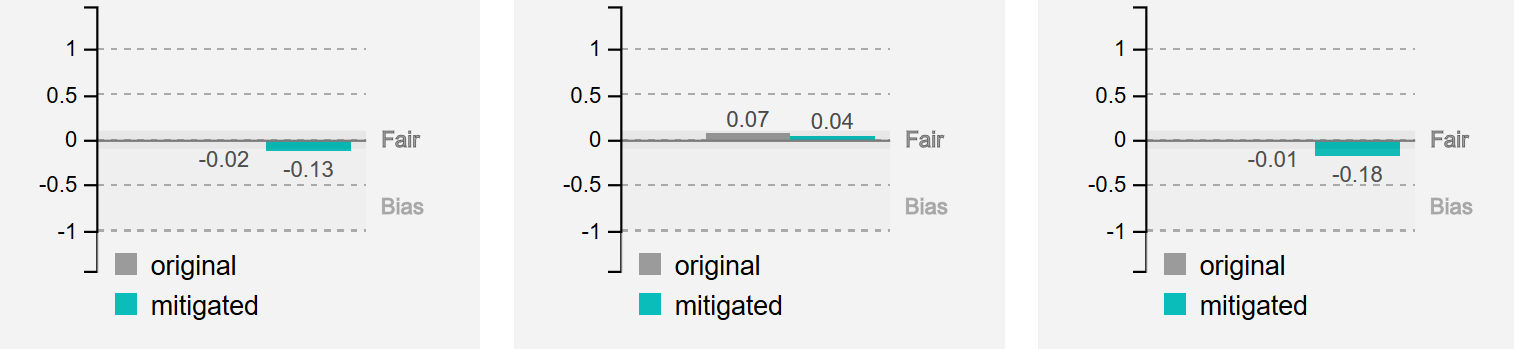
\includegraphics[width=\linewidth,height=25mm]{images/debias_3.png}
		\caption{Privileged male and unprivileged female groups}
		 \label{fig:debias_3}
	\end{subfigure}
	\begin{subfigure}{0.48\linewidth}
		\centering
		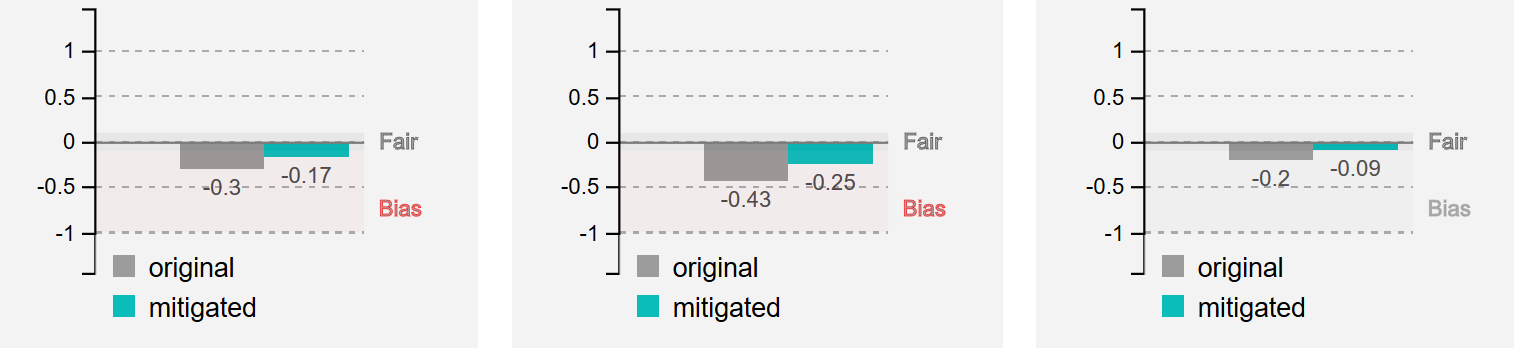
\includegraphics[width=\linewidth,height=24mm]{images/debias_4.png}
		\caption{Privileged 'white' and unprivileged 'black' groups}
        \label{fig:debias_4}
	\end{subfigure}
	\caption{Bias mitigation using adversarial debiasing algorithm, where statistical parity difference, equal opportunity difference, and average odds difference are shown}
	\label{fig:debiases_2}
	\vspace{-2mm}
\end{figure*}
\fi 

\subsection{Generating and explaining with fair decision rules}
\label{sec:rule_gen_inter}
Previously, we generate decision rules using RuleMatrix and Skater, and explain the cancer diagnosis in an intuitive way. As discussed, we rely on Bayesian optimization and statistical approaches to generate those rules. Now that we have the rules, none of the rules are backed by the domain knowledge. In symbolic AI or Good Old-Fashioned Artificial Intelligence~(GOFAI)~\cite{GoFI}, real-world knowledge is not derived by mathematical optimization, but hard-coded in the system exploiting formal languages~\cite{futia2020integration}. To develop a robust CDSS, it is crucial to understand its weakness, e.g., why and in what circumstance it will fail. Besides, to rectify mistakes and biases decisions, we expect to have the full control of the system. 

\subsubsection{Generating fair decision rules}
Inspired by these, we hypothesize\footnote{\textbf{H6}: Fair decision rules can be deduced by combining predictions and the reasoning.} that symbolic decision rules based on ontological reasoning and backed by the domain knowledge and description logic~(DLx) will be fairer, st. we not only rely on the model predictions, but also interpretation, e.g., feature attributions and reasoning. 
%irst, we collect initial prediction by the model~(including misclassified instances), before we observe individual rule and performing reasoning. 
%Subsequently, we identify the difference made by the model and the reasoning by the reasoner. 
%In order to generate fair decision rules, first, 
The model is evaluated on the test set. Then individual predictions are observed, before identifying both correctly and misclassified instances. The list of top-k genes is then created based on feature importance, followed by grouping them into oncogenes, protein-coding, and POTSF genes. The Bayesian rule set~(rule-base) for each prediction is then generated. Then, for each rule, we create a list of each antecedent and the prediction, followed by querying KG via a semantic reasoner for each biomarker.

\hspace*{3.5mm} Each matched biomarker extracted from the  DLx query is then identified, followed by inferring the rules \footnote{Using DLx class axiom render} and identifying the degree of significance and evidence~(e.g., PubMed). Subsequently, the rule updater updates the final rule set, where each rule is modified by combining degree of significance and evidence as additional antecedents, if available. Finally, the explanation in the interactive explanations module is updated. \Cref{algo:fair_dr} shows the procedure for generating fair decision rules. 

\iffalse
%\vspace{-2mm}
\begin{itemize}[noitemsep]
    \item \textbf{Step -1}: We evaluate the model on the test set as well as we observe individual predictions and identify both correctly and misclassified instances. 
    \item \textbf{Step-2}: We create a list of top-k genes based on the feature importance and group them as oncogenes, protein-coding, and POTSF genes. 
    \item \textbf{Step-3}: Create the Bayesian rule set~(rule-base for our CDSS) for each prediction in step-1.
    \item \textbf{Step-4}: For each rule, create a dictionary of each antecedent and corresponding prediction. 
    \item \textbf{Step-5}: Query the KG via a semantic reasoner and search each biomarker. 
    \item \textbf{Step-6}: List each matched biomarker based on the DLx query. 
    \item \textbf{Step-7}: Use the DLx class axiom render to infer rule for each biomarker and identify the degree of significance and evidence~(e.g., PubMed) association. 
    \item \textbf{Step-8}: Update the final rule set in the rule-based explanation module, where we modify each rule by combining degree of significance and evidence association as additional antecedents. 
    \item \textbf{Step-9}: Update the explanation in the interactive explanations module. 
\end{itemize}
\fi 

%\vspace{-2mm}
\begin{algorithm*}[h]
\caption{Generating fair decision rules}
\small{
    \DontPrintSemicolon \SetKwInOut{Input}{Input}%
      \SetKwInOut{Output}{Output}%
      \Input{An Oracle model $\mathcal{M}^{o}$ trained on multimodal genomics data.}%
      \Output{Fair decision rules $\mathcal{R}^{f}$ for a Bayesian rule set $\mathcal{R}^{b}$}%
      \textbf{Step-1}: Evaluate model $\mathcal{M}$ on the test set and generate individual predictions $\mathcal{P}$. \\
      \textbf{Step-2}: Create the list of top-k genes $\mathcal{T}$ based on feature importance and group into oncogenes, protein-coding, and POTSF genes.\\
      \textbf{Step-3}: Create a surrogate model $\mathcal{M}^{s}$ to approximate $\mathcal{M}^{o}$.\\
      \textbf{Step-4}: Create the Bayesian rule set $\mathcal{R}^b$ for each prediction $p_i \in \mathcal{P}$.\\
      \BlankLine%
     \For{$r_i \in \mathcal{R}^b$}{ \tcp*{Step-5: for each rule do}
            $\mathcal{(A}, \mathcal{C}) \leftarrow  \{\}$ \tcp*{Dictionary of antecedent(s)~(single/multi biomarkers) and its prediction}\; 
            \vspace{-2mm}
            $ a_i \leftarrow {r_i}$.split(`if')\;
            $\mathcal{A} \leftarrow \mathcal{A} \cup a_i$\;
            $ c_i \leftarrow {r_i}$.split(`Predicted Label:')\;
            $\mathcal{C} \leftarrow \mathcal{C} \cup c_i$\;
            \textbf{Return} $(\mathcal{A}, \mathcal{C})$
     }
     \For{$a_i \in \mathcal{A}$ and $c_i \in \mathcal{C}$}{
            $\mathcal{(S}, {E}) \leftarrow  \{\}$ \tcp*{Dictionary of degree of significance and evidence for each biomarker}\; 
            \vspace{-2mm}
            %\If{$F_i < \sigma $}{ \tcp*{If the feature importance is less than MAI}\;}
            \textbf{Step-6}: Query KG via reasoner and search each biomarker $a_i \in \mathcal{A}$. \\
            \textbf{Step-7}: List each matched biomarker $a_m$ \\
            \If{$a_m \in KG $}{\tcp*{Infer rule for each biomarker}\;
            \vspace{-4mm}
            $ s_i \leftarrow$ hasSignificance($a_m$)\;
            $\mathcal{S} \leftarrow \mathcal{S} \cup s_i$\;
            $ e_i \leftarrow$ hasEvidence($a_m$)\;
            ${E} \leftarrow {E} \cup e_i$\;
            \textbf{Return} $(\mathcal{S}, {E})$
            }
            %\textbf{Step-8}: Infer rule for each biomarker and identify the degree of significance and evidence~(e.g., PubMed) association. \\
            \textbf{Step-9}: Update rule set by combining degree of significance and evidence association: \\
            $\mathcal{R}^{f} \leftarrow \mathcal{R}^{b} \cup (\mathcal{S}, {E})$\\
            %Update the final rule set in the rule-based explanation module, where we modify each rule by combining degree of significance and evidence association as additional antecedents. \\
            %\textbf{Step-10}: Update the explanation in the interactive explanations module. 
            \textbf{Return} $\mathcal{R}^{f}$
     }}
     \label{algo:fair_dr}
\end{algorithm*}

\begin{itemize}[noitemsep]
\scriptsize{
    \item TP53 $ \sqsubseteq  $ Biomarker
    \item TP53 $ \sqsubseteq  $ $  \forall $is$ {\_}$a.Protein-coding
    \item TP53 $ \sqsubseteq  $ $  \forall $is$ {\_}$a.POTSF
    \item TP53 $  \cap $ ($\exists$has$ {\_}$significance$ {\_}$degree.High) $  \cap $ ($\exists$responsible$ {\_}$for.BreastCancer) $ \sqsubseteq  $ ($\exists$has$ {\_}$evidence.PubMed) $\cap$ (=493) (has ${\_}$citations.T)}
\end{itemize}

%\vspace{-2mm}
\begin{itemize}[noitemsep]
\scriptsize{
    \item AKT1 $ \sqsubseteq  $ Biomarker
    \item AKT1 $ \sqsubseteq  $ $\exists$is$ {\_}$a.Oncogene
    \item AKT1 $ \sqsubseteq  $ ($\exists$has$ {\_}$significance$ {\_}$degree.High) $  \cap $ ($\exists$responsible$ {\_}$for.PanCan)
    \item AKT1 $ \sqsubseteq  $ ($\exists$has$ {\_}$evidence.PubMed) $  \cap $ ($\exists$has$ {\_}$significance$ {\_}$degree.Low) $  \cap $ ($\exists$responsible$ {\_}$for.UrinaryBladderCancer)
    \item AKT1 $ \sqsubseteq  $ ($\exists$has$ {\_}$significance$ {\_}$degree.Medium) $  \cap $ ($\exists$responsible$ {\_}$for.EndometrialCancer).}
\end{itemize}
%\vspace{-2mm}

\subsubsection{Interpreting fair decision rules}
\iffalse
To be finished ... 
IF (ModelPred == BRCA) AND IF TopKGenes IN (TP53, GATA3, MLL3, …) AND IF AVG\_FI >= 0.7 AND Top1Gene IS (Oncogene) PRED = BRCA

IF (ModelPred == COAD) AND IF TopKGenes IN (EPHA6, TIMP1, ART5, …) AND IF GeneSIG IN (HIGH, MEDIUM) PRED == COAD 

IF (ModelPred == KIRC) AND IF TopKGenes IN (EPHA6, TIMP1, ART5 …) AND IF AVG\_FI <= 0.45 PRED = LUAD

Generating decision rules for evidence: 
IF (ModelPred == BRCA) AND IF NUM\_PMID >= 2 AND IF AVG\_FI >= 0.7 PRED = BRCA
\fi 

Now relating this rule set with the decision rules can be described with an example. Suppose, a doctor uploads patient's multimodal genomic data~(or unimodal in restrictive scenario) to get the diagnosis decision. Based on the outcome at hand~(e.g., prediction, feature importance, decision rule set), he then can be ensured that the patient has breast cancer. Subsequently, he can explain that the model made such decision by exposing blood biomarkers role, e.g., TP53 is the most significant biomarkers. Further, upon the patient request, doctor can then write a SPARQL or DLx query and ask the reasoner to reason how the decision is deduced/inferred based on the following rules and domain-knowledge he is aware of:  

\begin{itemize}[noitemsep]
\scriptsize{
    \item TP53 $ \sqsubseteq  $ Biomarker
    \item TP53 $ \sqsubseteq  $ $  \forall $is$ {\_}$a.Protein-coding
    \item TP53 $ \sqsubseteq  $ $  \forall $is$ {\_}$a.POTSF
    \item TP53 $  \cap $ ($\exists$has$ {\_}$significance$ {\_}$degree.High) $  \cap $ ($\exists$responsible$ {\_}$for.BreastCancer) $ \sqsubseteq  $ ($\exists$has$ {\_}$evidence.PubMed) $\cap$ (=493) (has ${\_}$citations.T)}
\end{itemize}

\hspace*{3.5mm} Additionally, the doctor can interpret this rule to the patient, where the decision is backed by the fact that a gene biomarker called `TP53': `TP53' is found to be highly responsible for the presence of breast cancer in your body. This gene has very strong mutations associations w.r.t. to breast cancer. Nevertheless, many scientific article has found it's association. What we assume that such an inferred rule can be used not only to fix inconsistencies, but also to generate fairer decision rules.

\section{Chapter Summary}\label{chapter_9:conclusion}
In this chapter, attempts were taken to mitigate different types of bias such as sampling, reporting, and model selection bias. Besides, random forest classifier is  trained on individual modality to calculate feature importance by reducing biases and increasing variance. Besides, to understand clinical feature contributions to support the statistical feature importance, SHAP is employed in a post-hoc manner. Further, an attempt is taken to mitigate biases in automatic decision making as well as heterogeneity that could occur during the predictive modelling. Finally, the predictions were combined with the reasoning to generate fair decision rules. 

%Although fairness is an incredibly desirable quality from both clinical, technological, or philosophical side, it has been found that it is surprisingly difficult to make a CDSS fully fair. 
\hspace*{3.5mm} More specifically, several experiments were carried out to improve the adversarial robustness of the models, with the following objectives:

\begin{enumerate}[noitemsep]
    \item Can we train a surrogate model to approximate the behaviour of a complex DNN model? 
    \item How effective a surrogate model at approximating the oracle model?  
    \item How effective decision rules are to explain global and local behaviours of a model?   
    \item Can we explain misclassified instances using decision rules? 
\end{enumerate}

\hspace*{3.5mm} Results of each observation are analysed, both quantitative and qualitatively, in the following section.

\hspace*{3.5mm} There are three potential limitations of our approach w.r.t. fairness: i) we could not focus on other types of biases such as automation and coverage biases, which is mainly due to the nature of the data and experiment, ii) we could not yet externally validated or assessed our CDSS against the fairness, iii) we haven't computed any fairness metrics, hence we can't confidently say how fair our approach is. Now that we came to an end of the explainable journey towards developing a diagnosis decision support system, we should summarize the key findings and limitations before providing potential outlooks. In the next chapter, we conclude this thesis by discussing the overall key findings. Additionally, we'll provide several future research directions for the scientific communities. 



